% !TeX root = main.tex
\lecture{1}{Fri 03 Oct 2025 12:00}{Atomic Structure}

\subsection*{What is the course?}
\begin{itemize}
    \item Quantum mech is weird and unintuative, we will build up a case in the course for why this weird theory was necessary and why we're confident it works.
    \item Each week will be a self-contained concept and/or historial experiment, working up to the Shroedinger Equation and wave-particle duality.
    \item Names and dates do not need to be memorised.
    \item Recommended text: University Physics (Young and Freedman).
    \item Office hours: 13:00 -- 13:50 Fridays (immediately post-lecture), Physics East Rm 207.
\end{itemize}

\subsection*{Atomic Structure}
What actually is an atom? What does it actually look like inside?

\textbf{Early Clues}
\begin{itemize}
    \item Periodic Table (Mendelev, 1989), periodic patterns in elements properties.
    \item Radioactivity (Becquerel, 1896, Curie 1898)
    \item Atoms emit and absorb specific discrete wavelengths, (Balmer, 1884)
    \item Discovery of the Electron (Thompson 1897). Cathode rays - heating metal in a vacuum with an electric field above it, to strip away electrons from the metal.
    \begin{itemize}
        \item This showed electrons were negatively charged and extremely light (1/2000th of the atomic mass).
    \end{itemize}
\end{itemize}
\begin{figure}[H]
    \centering
    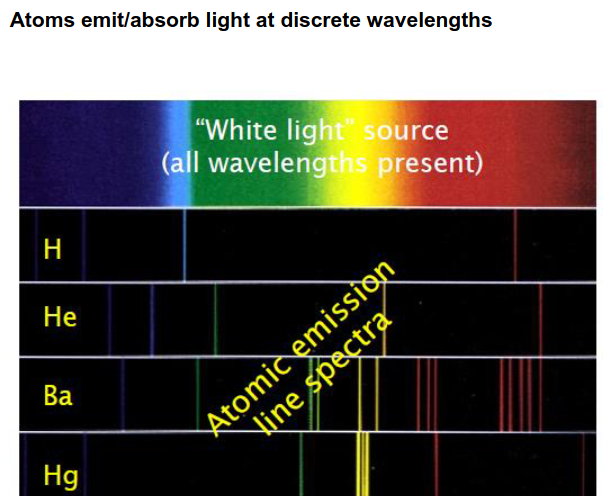
\includegraphics{figures/absorption_spectra.png}
     \caption{Absorption Spectra}
\end{figure}

\subsection*{Plum Pudding Model}
A solid, uniform lump of positively charged matter, approximately $10^{-10}$m across. This had evenly distributed negative charges (electrons) scattered throughout.

\subsection*{Discovery of the Nucleus}
Geiger and Marsden (1908-1913), fired alpha particles (He nuclei) at thin gold foil and measured the deflection / scattering.

The alpha particles had a mass of 4u, a charge of +2e and an energy of approximately 5MeV.

They found that most $\alpha$ were scattered only by small angles, but (surprisingly) a small number were scattered right back towards to emitter (through $\theta > 90\deg$). The distribution of the angles is approximately Normally distributed, with a mean of 0. Only approximately 1 in 8,000 fired $\alpha$s were scattered by $\theta>90$ ("back-scattering").

Can this be explained with the Plum Pudding Model? No, it cannot. This was used to demonstrate that atoms cannot be evenly distributed.

\section*{Demonstrating by Calculation}
Lets work out the work done to take an $\alpha$ from infty to the pudding centre. If the electrostatic repulsion is not enough to overcome this, we cannot stop the $\alpha$ and cannot back scatter.

\begin{figure}[H]
    \centering
    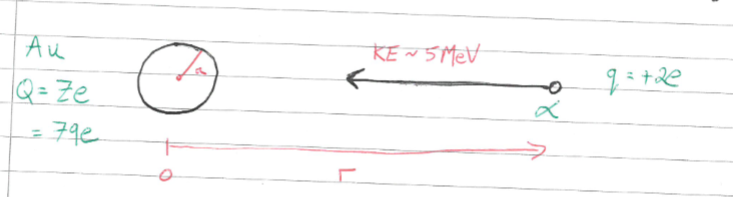
\includegraphics{figures/scattering.png}
     \caption{The experiment}
\end{figure}

\subsection*{Assumptions}
\begin{itemize}
    \item The atom stays still.
    \item Ignore the gold electrons (this is fine, as they would cancel some positive charge and make repulsion weaker, which would be even worse. If we can't do it without them, it would be equally impossible to do it with.)
\end{itemize}

\subsection*{Recap and Eqns}
 
Coulomb Potential Energy is:
\[
    u(r) - \frac{qQ}{4 \pi \epsilon_0 r}
\]

Force is:
\[
    F(r) = -\frac{du}{dr} = \frac{qQ}{4 \pi \epsilon_0 r^2}
\]

Change in potential energy ($u_2 - u_1$) is work done:
\[
    \int_{u_1}^{u_2} du = -\int_{r_1}^{r_2} F(r) dr
\]

From outside the atomic radius, we treat the atomic pudding as a point charge of charge Q.
From inside the atomic radius, we treat it as a smaller point charge $Q'(r)$, where we only consider the charge inside the portion of the pudding where $r<a$, where $a$ is the current position inside the sphere.

If charge is spread uniformly, the total charge is proportional to the volume of the sphere. So:
\[
    \frac{Q'}{Q} = \frac{\frac{4}{3} \pi r^3}{\frac{4}{3} \pi a^3}
\]
\[
    Q' = Q\frac{r^3}{a^3}
\]

\textbf{Inside the Pudding}
\[
    F = \frac{qQ'}{4 \pi \epsilon_0 r^2}
\]

\[
    F = \frac{qQr^3}{4 \pi \epsilon_0 r^2 a^3}
\]

\[
    F = \frac{qQr}{4 \pi \epsilon_0 a^3}
\]

\[
    F = \frac{qQ}{4 \pi \epsilon_0 a^3} \times r
\]


Hence inside, $F \propto r$

\textbf{Outside the Pudding}
\[
    F = \frac{Qq}{4 \pi \epsilon_0 r^2}
\]

\[
    F = \frac{Qq}{4 \pi \epsilon_0} \times \frac{1}{r^2}
\]


Hence outside, $F \propto \frac{1}{r^2}$

To integrate, we are therefore integrating the area under this (almost) triangle:
\begin{figure}[H]
    \centering
    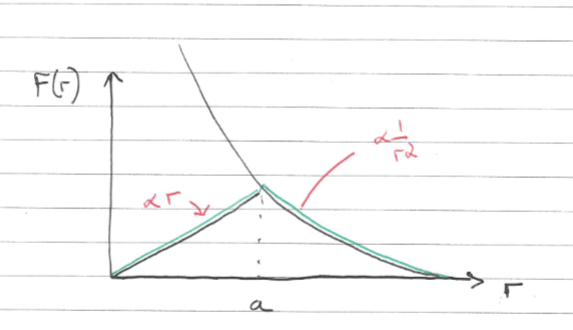
\includegraphics{figures/lec01-03.png}
     \caption{Radius vs electrostatic repulsion force }
\end{figure}

\[
    \Delta u = - \int_{r_1}^{r_2} F(r) \, dx
\]

Splitting into two sections (prior to, and after the point where r = atomic radius, $r = a$), and integrating across all r (as we are attempting to work out the work done to bring an $\alpha$ from infinity to the charge, at which poind distance is 0):
\[
    = -\int_{\infty}^{a} \frac{qQ}{4 \pi \epsilon_0 r^2} \, dx - \int_{a}^{0} \frac{qQr}{4 \pi \epsilon_0 a^3} \, dx
\]

\[
    = -\frac{qQ}{4 \pi \epsilon_0}\int_{\infty}^{a} \frac{1}{r^2} \, dx - \frac{qQ}{4 \pi \epsilon_0 a^3}\int_{a}^{0} r \, dx
\]

\[
    = -\frac{qQ}{4 \pi \epsilon_0} \lim_{x \to \infty} \int_{x}^{a} \frac{1}{r^2} \, dx - \frac{qQ}{4 \pi \epsilon_0 a^3}\int_{a}^{0} r \, dx
\]

\[
        = -\frac{qQ}{4 \pi \epsilon_0} \lim_{x \to \infty} \left[- \frac{1}{r}\right]_x^a - \frac{qQ}{4 \pi \epsilon_0 a^3} \left[\frac{1}{2}r^2\right]_a^0
\]

\[
        = -\frac{qQ}{4 \pi \epsilon_0} \left(-\frac{1}{a} - 0\right) - \frac{qQ}{4 \pi \epsilon_0 a^3} \left(\frac{1}{2}0^2 - \frac{1}{2}a^2\right)
\]

\[
        = -\frac{qQ}{4 \pi \epsilon_0} \left(-\frac{1}{a}\right) - \frac{qQ}{4 \pi \epsilon_0 a^3} \left(- \frac{1}{2}a^2\right)
\]

\[
    = \frac{qQ}{4 \pi \epsilon_0 a} + \frac{qQa^2}{8 \pi \epsilon_0 a^3}
\]

\[
    = \frac{qQ}{4 \pi \epsilon_0 a} + \frac{qQ}{8 \pi \epsilon_0 a}
\]

\[
    = \frac{qQ}{4 \pi \epsilon_0 a} + \frac{1}{2}\frac{qQ}{4 \pi \epsilon_0 a}
\]

\[
    = \frac{3}{2}\frac{qQ}{4 \pi \epsilon_0}
\]
As required! Plugging in values gives us:
\[
    \Delta u = \frac{3}{2} \frac{(2e)(79e)}{4 \pi (8.854 \times 10^{-12}) \times 10^{-10}}
\]
\[
    = 5.45 \times 10^{-16}J = 3.41KeV
\]
This is much less than the kinetic energy of the 5MeV alpha particle, therefore (as this value is maximum work done against the repulsive force) a plum pudding could not backscatter a 5MeV alpha particle. However, since $\Delta u \propto 1/a$, a smaller volume of charge could. How small, however?

\[
    \Delta u = 5 \text{MeV} = -\int_{\infty}^{r_{max}} \frac{qQ}{4 \pi \epsilon_0 r^2} \, dr
\]

\[
    -5 \text{MeV} = \frac{qQ}{4 \pi \epsilon_0}\int_{\infty}^{r_{max}} \frac{1}{r^2} \, dr
\]

\[
    -5 \text{MeV} = \frac{qQ}{4 \pi \epsilon_0} \lim_{x \to \infty} \left[ - \frac{1}{r}\right]^{r_{max}}_x
\]
\[
    -5 \text{MeV} = \frac{qQ}{4 \pi \epsilon_0} \left[ -\frac{1}{r_{max}} - \lim_{x \to \infty} \frac{1}{x}\right]
\]

\[
    -5 \text{MeV} = \frac{qQ}{4 \pi \epsilon_0} \left[ -\frac{1}{r_{max}}\right]
\]

\[
    5 \text{MeV} = \frac{qQ}{4 \pi \epsilon_0 r_{\text{max}}}
\]

Subsitution and rearrangement gives $r_{\text{max}} = 4.5 \times 10^{-14}m = 45fm$.
We accept the $10^{-10}\text{m} = 100,000 \text{fm}$ figure as the total width of the atom, but this demonstrates that there must exist a nucleus of no larger than 45fm.

\subsection*{Next Idea: The Solar System Model}
Therefore, the next idea was an orbiting solar system model, where electrons orbit in fixed paths around a central nucleus. However, accelerating charges (i.e. a charge in circular motion) radiates energy, so this orbiting electron would be on a decaying path to crash into the nucleus. We can observe this does not happen, so need another idea\dots

Bohr made two postulates:
\begin{itemize}
    \item The electron in hydrogen moves in a set non-radiating circular orbit.
    \item Radiation is only emitted or abosrbed when an electron moves from one orbit to another.
\end{itemize}

This works (at least for hydrogen) and explains the absoption spectra, but for now lacks a physical grounding.